
%(BEGIN_QUESTION)
% Copyright 2006, Tony R. Kuphaldt, released under the Creative Commons Attribution License (v 1.0)
% This means you may do almost anything with this work of mine, so long as you give me proper credit

Identify the type of {\it filter circuit} (LP, HP, BP, or BS) with the following frequency response:

$$\includegraphics[width=15.5cm]{i00630x01.eps}$$

Now, sketch a schematic diagram for a filter circuit exhibiting this response:

$$\includegraphics[width=15.5cm]{i00630x03.eps}$$

\vskip 20pt \vbox{\hrule \hbox{\strut \vrule{} {\bf Suggestions for Socratic discussion} \vrule} \hrule}

\begin{itemize}
\item{} Is there more than one circuit topology exhibiting this type of frequency response?  If so, identify at least one other design that will respond the same way.
\end{itemize}

\underbar{file i00630}
%(END_QUESTION)





%(BEGIN_ANSWER)

\noindent
{\bf Partial answer:}

This filter is also known as a {\it notch} filter.  I'll let you figure out which of the four abbreviated filter types is a synonym for ``notch filter.''

\vskip 10pt

Here is one possible schematic diagram for a notch filter circuit:

$$\includegraphics[width=15.5cm]{i00630x02.eps}$$

\vskip 10pt

Follow-up question: how would you calculate the notch frequency of this filter circuit?

%(END_ANSWER)





%(BEGIN_NOTES)

$$f_{notch} = {1 \over {2 \pi \sqrt{LC}}}$$

%INDEX% Electronics review: filter circuit

%(END_NOTES)


